% Options for packages loaded elsewhere
\PassOptionsToPackage{unicode}{hyperref}
\PassOptionsToPackage{hyphens}{url}
%
\documentclass[
]{article}
\usepackage{amsmath,amssymb}
\usepackage{iftex}
\ifPDFTeX
  \usepackage[T1]{fontenc}
  \usepackage[utf8]{inputenc}
  \usepackage{textcomp} % provide euro and other symbols
\else % if luatex or xetex
  \usepackage{unicode-math} % this also loads fontspec
  \defaultfontfeatures{Scale=MatchLowercase}
  \defaultfontfeatures[\rmfamily]{Ligatures=TeX,Scale=1}
\fi
\usepackage{lmodern}
\ifPDFTeX\else
  % xetex/luatex font selection
\fi
% Use upquote if available, for straight quotes in verbatim environments
\IfFileExists{upquote.sty}{\usepackage{upquote}}{}
\IfFileExists{microtype.sty}{% use microtype if available
  \usepackage[]{microtype}
  \UseMicrotypeSet[protrusion]{basicmath} % disable protrusion for tt fonts
}{}
\makeatletter
\@ifundefined{KOMAClassName}{% if non-KOMA class
  \IfFileExists{parskip.sty}{%
    \usepackage{parskip}
  }{% else
    \setlength{\parindent}{0pt}
    \setlength{\parskip}{6pt plus 2pt minus 1pt}}
}{% if KOMA class
  \KOMAoptions{parskip=half}}
\makeatother
\usepackage{xcolor}
\usepackage[margin=1in]{geometry}
\usepackage{color}
\usepackage{fancyvrb}
\newcommand{\VerbBar}{|}
\newcommand{\VERB}{\Verb[commandchars=\\\{\}]}
\DefineVerbatimEnvironment{Highlighting}{Verbatim}{commandchars=\\\{\}}
% Add ',fontsize=\small' for more characters per line
\usepackage{framed}
\definecolor{shadecolor}{RGB}{248,248,248}
\newenvironment{Shaded}{\begin{snugshade}}{\end{snugshade}}
\newcommand{\AlertTok}[1]{\textcolor[rgb]{0.94,0.16,0.16}{#1}}
\newcommand{\AnnotationTok}[1]{\textcolor[rgb]{0.56,0.35,0.01}{\textbf{\textit{#1}}}}
\newcommand{\AttributeTok}[1]{\textcolor[rgb]{0.13,0.29,0.53}{#1}}
\newcommand{\BaseNTok}[1]{\textcolor[rgb]{0.00,0.00,0.81}{#1}}
\newcommand{\BuiltInTok}[1]{#1}
\newcommand{\CharTok}[1]{\textcolor[rgb]{0.31,0.60,0.02}{#1}}
\newcommand{\CommentTok}[1]{\textcolor[rgb]{0.56,0.35,0.01}{\textit{#1}}}
\newcommand{\CommentVarTok}[1]{\textcolor[rgb]{0.56,0.35,0.01}{\textbf{\textit{#1}}}}
\newcommand{\ConstantTok}[1]{\textcolor[rgb]{0.56,0.35,0.01}{#1}}
\newcommand{\ControlFlowTok}[1]{\textcolor[rgb]{0.13,0.29,0.53}{\textbf{#1}}}
\newcommand{\DataTypeTok}[1]{\textcolor[rgb]{0.13,0.29,0.53}{#1}}
\newcommand{\DecValTok}[1]{\textcolor[rgb]{0.00,0.00,0.81}{#1}}
\newcommand{\DocumentationTok}[1]{\textcolor[rgb]{0.56,0.35,0.01}{\textbf{\textit{#1}}}}
\newcommand{\ErrorTok}[1]{\textcolor[rgb]{0.64,0.00,0.00}{\textbf{#1}}}
\newcommand{\ExtensionTok}[1]{#1}
\newcommand{\FloatTok}[1]{\textcolor[rgb]{0.00,0.00,0.81}{#1}}
\newcommand{\FunctionTok}[1]{\textcolor[rgb]{0.13,0.29,0.53}{\textbf{#1}}}
\newcommand{\ImportTok}[1]{#1}
\newcommand{\InformationTok}[1]{\textcolor[rgb]{0.56,0.35,0.01}{\textbf{\textit{#1}}}}
\newcommand{\KeywordTok}[1]{\textcolor[rgb]{0.13,0.29,0.53}{\textbf{#1}}}
\newcommand{\NormalTok}[1]{#1}
\newcommand{\OperatorTok}[1]{\textcolor[rgb]{0.81,0.36,0.00}{\textbf{#1}}}
\newcommand{\OtherTok}[1]{\textcolor[rgb]{0.56,0.35,0.01}{#1}}
\newcommand{\PreprocessorTok}[1]{\textcolor[rgb]{0.56,0.35,0.01}{\textit{#1}}}
\newcommand{\RegionMarkerTok}[1]{#1}
\newcommand{\SpecialCharTok}[1]{\textcolor[rgb]{0.81,0.36,0.00}{\textbf{#1}}}
\newcommand{\SpecialStringTok}[1]{\textcolor[rgb]{0.31,0.60,0.02}{#1}}
\newcommand{\StringTok}[1]{\textcolor[rgb]{0.31,0.60,0.02}{#1}}
\newcommand{\VariableTok}[1]{\textcolor[rgb]{0.00,0.00,0.00}{#1}}
\newcommand{\VerbatimStringTok}[1]{\textcolor[rgb]{0.31,0.60,0.02}{#1}}
\newcommand{\WarningTok}[1]{\textcolor[rgb]{0.56,0.35,0.01}{\textbf{\textit{#1}}}}
\usepackage{graphicx}
\makeatletter
\newsavebox\pandoc@box
\newcommand*\pandocbounded[1]{% scales image to fit in text height/width
  \sbox\pandoc@box{#1}%
  \Gscale@div\@tempa{\textheight}{\dimexpr\ht\pandoc@box+\dp\pandoc@box\relax}%
  \Gscale@div\@tempb{\linewidth}{\wd\pandoc@box}%
  \ifdim\@tempb\p@<\@tempa\p@\let\@tempa\@tempb\fi% select the smaller of both
  \ifdim\@tempa\p@<\p@\scalebox{\@tempa}{\usebox\pandoc@box}%
  \else\usebox{\pandoc@box}%
  \fi%
}
% Set default figure placement to htbp
\def\fps@figure{htbp}
\makeatother
\setlength{\emergencystretch}{3em} % prevent overfull lines
\providecommand{\tightlist}{%
  \setlength{\itemsep}{0pt}\setlength{\parskip}{0pt}}
\setcounter{secnumdepth}{-\maxdimen} % remove section numbering
\usepackage{bookmark}
\IfFileExists{xurl.sty}{\usepackage{xurl}}{} % add URL line breaks if available
\urlstyle{same}
\hypersetup{
  pdftitle={Lab 01 - Introduction to R and R Markdown},
  hidelinks,
  pdfcreator={LaTeX via pandoc}}

\title{Lab 01 - Introduction to R and R Markdown}
\author{}
\date{\vspace{-2.5em}2025-09-02}

\begin{document}
\maketitle

{
\setcounter{tocdepth}{2}
\tableofcontents
}
\section{Getting Started with R
Markdown}\label{getting-started-with-r-markdown}

This is an R Markdown document.

At present, you are reading it formatted as an HTML document, but as we
have seen, it can also be rendered as a PDF -- when working with an .Rmd
file, you can choose how it is presented by selecting the arrow next to
the Knit ball of yarn an choose between ``Knit to HTML'' or ``Knit to
PDF''. For most of the work in this class, we will be knitting to a PDF
to facilitate submissions to canvas.

When you Knit an R Markdown file, it will ask you to first save and name
your document. I recommend sticking to a consistent format throughout
the semester: something like \texttt{lastname\_{[}lab/hwk{]}\_\#.Rmd}.
For example, I would name this \texttt{paris\_lab\_1.Rmd}. After you
knit, this will also be the name of your pdf.

For this lab, we will be following along with this document which we can
begin by downloading the .Rmd file associated with it
\href{01_introR.Rmd}{here}; this is allow us to see side-by-side how the
.Rmd file looks compared to the finished output.

For example, reading this online we see that \textbf{this sentence is
bold}, while in the .Rmd file we see that the sentence is a plain-text
sentence surrounded by two asterisks (**) on each side. This is an
example of using
\href{https://www.markdownguide.org/basic-syntax/}{markdown} to format
our documents. For this lab, we will be following along with the .Rmd
file, filling bits in as prompted. Let's begin by introducing some of
the more common markdown syntax that we will use in this class.

\subsection{Text Editing}\label{text-editing}

We can use .Rmd files to write text just as we would with a standard
word processor. As we saw previously, using \textbf{two asterisks}
creates bold text, whereas using \emph{single asterisks} creates text
that is italicized.

Headers can be created using the \# symbol. Using one creates a large
header, two a smaller header, and so on. You can see examples of this in
the text above (this section on ``Text Editing'' uses two to create a
header). Take note that you need to leave a space between the \# and the
header text -- forgetting to do so will render the text exactly as you
have written it.

\#For example, this will not show up as a header

We can also create sequential lists. To do so, start new lines with
sequential numbers

\begin{enumerate}
\def\labelenumi{\arabic{enumi}.}
\tightlist
\item
  Like this
\item
  And this
\item
  And finally this
\end{enumerate}

We can create un-ordered lists with using stars or dashes

\begin{itemize}
\tightlist
\item
  Here is an item
\item
  Here is another item

  \begin{itemize}
  \tightlist
  \item
    And if I indent, I can make nested lists
  \end{itemize}
\end{itemize}

We can also create horizontal dividers with a line of stars (at least 3,
but any number greater is ok). This is a good way to separate your
answers from a given problem

\begin{center}\rule{0.5\linewidth}{0.5pt}\end{center}

Things are more clear if I put my answers between bars, but I need to be
sure to leave a blank line between my text and the bottom star

\begin{center}\rule{0.5\linewidth}{0.5pt}\end{center}

\textbf{Question 1:}

Create a new R Markdown file and copy the entirety of this question over
to the new file (we will do this for all questions in this lab). Then,
proceed with the instructions below.

Between the stars below, do the following:

\begin{enumerate}
\def\labelenumi{\arabic{enumi}.}
\tightlist
\item
  Use two \# to create a header that says About Me
\item
  Type your first name in bold and your last name in italics
\item
  Create a bullet point list of the people sitting on either side of you
\item
  Create a numbered list of your 3 least favorite animals
\end{enumerate}

Once you have done this, Knit to PDF by clicking the bar of yarn above
and verify that everything looks like it should.

\begin{center}\rule{0.5\linewidth}{0.5pt}\end{center}

\begin{center}\rule{0.5\linewidth}{0.5pt}\end{center}

\section{Getting Started with R
Studio}\label{getting-started-with-r-studio}

Whereas R is the programming language responsible for doing our relevant
computation, our interactions with R will be primarily through R Studio.
When you first open R Studio, your screen will partitioned into 3 panes:
\emph{Console}, \emph{Environment}, and \emph{Files} (and often,
\emph{Editor})

\subsubsection{Console}\label{console}

The console makes up the lower left-hand side of the screen, and it is
here that we can interact with R directly. Some information will appear
on start-up, followed by a prompt (indicated with
\texttt{\textgreater{}}). Try copying and pasting the following lines
into your console one at a time and pressing enter:

5 + 2

sqrt(25)

pi

(3\^{}2 + 1)*5

x \textless- 5

\subsubsection{Environment}\label{environment}

The environment panel is located in the top right and includes all of
the named variables that we have created in R. If you copied the lines
above correctly, you should see a single line here, indicating that the
variable \texttt{x} has the value \texttt{5}. When starting a new R
session, this pane will be empty.

\subsubsection{Output/Files}\label{outputfiles}

In the bottom right is the Output pane which, in addition to giving us
information about our file system also includes tabs for Plots and Help.
Copy each of the lines below to see how this pane changes

?sqrt

plot(1:10)

You can click any of the tabs in this pane to change what is currently
being shown.

\subsubsection{Editor}\label{editor}

Finally, we have the editor. If you start a new R Studio session, there
will be nothing in the editor, but this will change if we open either a
.R or .Rmd file. An R Script is the simplest type of file which can be
created from the menus at the top:

\begin{quote}
File -\textgreater{} New File -\textgreater{} R Script
\end{quote}

The editor pane will appear with a blank R file in which you can write
and store R code. Try copying the R commands from the \emph{Console}
section into an R Script, click on the line with code and click
``Ctrl+Enter'' on your keyboard. R Studio should execute this code and
display the results in the Console. You do not have to save this file,
and you can close it when you are finished.

\section{Getting Started with R}\label{getting-started-with-r}

While it is true that R scripts (files that end in .R) are used for the
vast majority of written R code, we will primarily be using R Markdown
files (files that end in .Rmd).

Perhaps the most obvious utility in using R Markdown documents for this
course is their ability to interweave regular text with R. We can
include and run R code by including it in a \emph{code chunk}, such as
the one shown below:

\begin{Shaded}
\begin{Highlighting}[]
\CommentTok{\# This is a code comment, beginning with \#}
\NormalTok{x }\OtherTok{\textless{}{-}} \DecValTok{4} 
\NormalTok{x}\SpecialCharTok{\^{}}\DecValTok{2}
\end{Highlighting}
\end{Shaded}

\begin{verbatim}
## [1] 16
\end{verbatim}

This code will run and display its results when we push the Knit button,
but we can also run the code without knitting by place by again clicking
the line with our cursor and hitting ``Ctrl+Enter''

For this portion of the lab, we will be introducing some of the basic
mechanics in the R language. This will include \texttt{vectors}, similar
to the variables we discussed in class, as well as \texttt{data.frames},
the primary data type we will be using for collections of observations.

You are welcome to follow along on the course website or read the R
Markdown directly. In either event, I highly encourage you to try
running the code that we see, either by coping it from the website and
pasting into the console, or by running with the R Markdown code chunks.

\subsection{Vectors}\label{vectors}

\subsubsection{Creating and subsetting}\label{creating-and-subsetting}

Vectors in R are the simplest type of object. Every vector has two
attributes that will dictate how we use it: length and type. We have
already seen vectors of length one, which are created by assigning a
number to a name using \texttt{\textless{}-}

\begin{Shaded}
\begin{Highlighting}[]
\CommentTok{\# This is a numeric vector of length 1}
\NormalTok{x }\OtherTok{\textless{}{-}} \DecValTok{4}
\NormalTok{x}
\end{Highlighting}
\end{Shaded}

\begin{verbatim}
## [1] 4
\end{verbatim}

We can create vectors of greater than length one using \texttt{c()},
which is short for ``combine''

\begin{Shaded}
\begin{Highlighting}[]
\NormalTok{y }\OtherTok{\textless{}{-}} \FunctionTok{c}\NormalTok{(}\DecValTok{2}\NormalTok{, }\DecValTok{4}\NormalTok{, }\DecValTok{6}\NormalTok{, }\DecValTok{8}\NormalTok{, }\DecValTok{10}\NormalTok{)}
\NormalTok{y}
\end{Highlighting}
\end{Shaded}

\begin{verbatim}
## [1]  2  4  6  8 10
\end{verbatim}

Sequences of vectors can also be created with \texttt{:}

\begin{Shaded}
\begin{Highlighting}[]
\NormalTok{z }\OtherTok{\textless{}{-}} \DecValTok{1}\SpecialCharTok{:}\DecValTok{5}
\NormalTok{z}
\end{Highlighting}
\end{Shaded}

\begin{verbatim}
## [1] 1 2 3 4 5
\end{verbatim}

Every element of a vector has a position that we can access directly
using square brackets \texttt{{[}{]}} in a process called
\emph{subsetting}. Here, we grab the 3rd element of the vector
\texttt{w}

\begin{Shaded}
\begin{Highlighting}[]
\NormalTok{w }\OtherTok{\textless{}{-}} \FunctionTok{c}\NormalTok{(}\DecValTok{3}\NormalTok{, }\DecValTok{6}\NormalTok{, }\DecValTok{9}\NormalTok{, }\DecValTok{12}\NormalTok{)}
\NormalTok{w[}\DecValTok{3}\NormalTok{]}
\end{Highlighting}
\end{Shaded}

\begin{verbatim}
## [1] 9
\end{verbatim}

\textbf{Question 2:}

Again, copy the entirety of this question into the R Markdown file you
created for Question 1.

Let's practice creating vectors and subsetting with a short exercise.

\begin{enumerate}
\def\labelenumi{\arabic{enumi}.}
\tightlist
\item
  First, create an R code chunk between the rows of stars below
  (Ctrl+Alt+I is quick way to do this)
\item
  Next, create a vector called \texttt{x} that has all of the numbers
  from 11 to 20
\item
  Use square brackets and subsetting to select the first five numbers of
  this vector.
\end{enumerate}

Note in R, like most programming languages, there are many ways to
accomplish any task. ****

\begin{center}\rule{0.5\linewidth}{0.5pt}\end{center}

\subsubsection{Vector types}\label{vector-types}

Just as we saw in class that variables can be quantitative or
categorical, so it is with vectors in R. There are primarily 3 types of
vectors we need to be aware of:

\begin{enumerate}
\def\labelenumi{\arabic{enumi}.}
\tightlist
\item
  \emph{numeric} - for example: \texttt{x\ \textless{}-\ c(1,\ 2,\ 3)}
\item
  \emph{character} - for example:
  \texttt{x\ \textless{}-\ c("a",\ "b",\ "c")}
\item
  \emph{logical} - for example
  \texttt{x\ \textless{}-\ c(TRUE,\ FALSE,\ TRUE)}
\end{enumerate}

Don't worry about memorizing everything -- we will continue to review
them together as they appear in the course. For now, we will be
satisfied with simply having made our introductions.

As we mentioned in class, the type of a variable will often dictate what
we are able to do with it. For example, it should make sense to take the
mean of a numeric variable, but less so with a character vector. We do
this using the R function \texttt{mean()}:

\begin{Shaded}
\begin{Highlighting}[]
\CommentTok{\# This will return a warning and NA (NA = Not Available/Missing Value)}
\NormalTok{z }\OtherTok{\textless{}{-}} \FunctionTok{c}\NormalTok{(}\StringTok{"a"}\NormalTok{, }\StringTok{"b"}\NormalTok{, }\StringTok{"c"}\NormalTok{)}
\FunctionTok{mean}\NormalTok{(z)}
\end{Highlighting}
\end{Shaded}

\begin{verbatim}
## Warning in mean.default(z): argument is not numeric or logical: returning NA
\end{verbatim}

\begin{verbatim}
## [1] NA
\end{verbatim}

\begin{Shaded}
\begin{Highlighting}[]
\NormalTok{x }\OtherTok{\textless{}{-}} \FunctionTok{c}\NormalTok{(}\DecValTok{1}\NormalTok{, }\DecValTok{2}\NormalTok{, }\DecValTok{3}\NormalTok{)}
\FunctionTok{mean}\NormalTok{(x)}
\end{Highlighting}
\end{Shaded}

\begin{verbatim}
## [1] 2
\end{verbatim}

Some situations can be confusing based on appearances. The
\texttt{class()} function will tell us what \emph{type} a vector is if
we are not sure

\begin{Shaded}
\begin{Highlighting}[]
\CommentTok{\# This looks numeric}
\NormalTok{z }\OtherTok{\textless{}{-}} \FunctionTok{c}\NormalTok{(}\StringTok{"1"}\NormalTok{, }\StringTok{"2"}\NormalTok{, }\StringTok{"3"}\NormalTok{)}
\NormalTok{z}
\end{Highlighting}
\end{Shaded}

\begin{verbatim}
## [1] "1" "2" "3"
\end{verbatim}

\begin{Shaded}
\begin{Highlighting}[]
\FunctionTok{mean}\NormalTok{(z)}
\end{Highlighting}
\end{Shaded}

\begin{verbatim}
## Warning in mean.default(z): argument is not numeric or logical: returning NA
\end{verbatim}

\begin{verbatim}
## [1] NA
\end{verbatim}

\begin{Shaded}
\begin{Highlighting}[]
\CommentTok{\# but actually, it is a character}
\FunctionTok{class}\NormalTok{(z)}
\end{Highlighting}
\end{Shaded}

\begin{verbatim}
## [1] "character"
\end{verbatim}

Usually in situations like this, we can \emph{coerce} a vector to being
a different type, though I will try to make you aware in advance when a
situation like this will arise:

\begin{Shaded}
\begin{Highlighting}[]
\CommentTok{\# coerce the z variable to be a numeric vector}
\NormalTok{z\_num }\OtherTok{\textless{}{-}} \FunctionTok{as.numeric}\NormalTok{(z)}
\NormalTok{z\_num}
\end{Highlighting}
\end{Shaded}

\begin{verbatim}
## [1] 1 2 3
\end{verbatim}

\begin{Shaded}
\begin{Highlighting}[]
\FunctionTok{class}\NormalTok{(z\_num)}
\end{Highlighting}
\end{Shaded}

\begin{verbatim}
## [1] "numeric"
\end{verbatim}

\begin{Shaded}
\begin{Highlighting}[]
\FunctionTok{mean}\NormalTok{(z\_num)}
\end{Highlighting}
\end{Shaded}

\begin{verbatim}
## [1] 2
\end{verbatim}

Deciding what class a vector should have is often context specific. For
example, having numeric vectors is ideal if we plan on using them for
mathematical operations (i.e., finding the mean, adding them together,
taking a square root), which may make sense for things like age,
population size, or temperature. Other times, a variable with numbers
may make more sense as a character vector to represent categories: this
could be things like room numbers, the year an automobile was
manufactured, or group assignments.

One important characteristic of a vector to note: all elements of a
vector \emph{must} be the same type. They are either all numeric, all
logical, or all character. R will force this by default:

\begin{Shaded}
\begin{Highlighting}[]
\NormalTok{z\_mix }\OtherTok{\textless{}{-}} \FunctionTok{c}\NormalTok{(}\StringTok{"a"}\NormalTok{, }\DecValTok{1}\NormalTok{, }\ConstantTok{TRUE}\NormalTok{)}

\DocumentationTok{\#\# They are all forced to be character}
\FunctionTok{class}\NormalTok{(z\_mix)}
\end{Highlighting}
\end{Shaded}

\begin{verbatim}
## [1] "character"
\end{verbatim}

\begin{Shaded}
\begin{Highlighting}[]
\CommentTok{\#we can try to force the class to be different }
\CommentTok{\#by assigning numeric to the class of z\_mix}
\FunctionTok{class}\NormalTok{(z\_mix) }\OtherTok{\textless{}{-}} \StringTok{"numeric"}
\end{Highlighting}
\end{Shaded}

\begin{verbatim}
## Warning in class(z_mix) <- "numeric": NAs introduced by coercion
\end{verbatim}

\begin{Shaded}
\begin{Highlighting}[]
\NormalTok{z\_mix}
\end{Highlighting}
\end{Shaded}

\begin{verbatim}
## [1] NA  1 NA
\end{verbatim}

\begin{Shaded}
\begin{Highlighting}[]
\CommentTok{\#No way to force "a" to be a number, not surprising}
\end{Highlighting}
\end{Shaded}

Characters are the most broad (ie least useful) of the data types and is
usually avoided when possible. Nominal variables in R are better
coverted to \emph{factors} which is an alterantive class. These will be
gone over later.

\subsection{Data Frames}\label{data-frames}

Most of the data we will be working with in this class will be stored in
objects known as data frames. Put simply, a data frame is a collection
of vectors that are all the same length.

\begin{Shaded}
\begin{Highlighting}[]
\CommentTok{\# Create two vectors of the same length}
\NormalTok{x }\OtherTok{\textless{}{-}} \FunctionTok{c}\NormalTok{(}\StringTok{"red"}\NormalTok{, }\StringTok{"green"}\NormalTok{, }\StringTok{"blue"}\NormalTok{)}
\NormalTok{y }\OtherTok{\textless{}{-}} \FunctionTok{c}\NormalTok{(}\DecValTok{1}\NormalTok{, }\DecValTok{4}\NormalTok{, }\DecValTok{10}\NormalTok{)}

\CommentTok{\# We can create a data frame with columns named \textasciigrave{}name\textasciigrave{} and \textasciigrave{}value\textasciigrave{}}
\NormalTok{df }\OtherTok{\textless{}{-}} \FunctionTok{data.frame}\NormalTok{(}\AttributeTok{name =}\NormalTok{ x, }\AttributeTok{value =}\NormalTok{ y)}

\NormalTok{df}
\end{Highlighting}
\end{Shaded}

\begin{verbatim}
##    name value
## 1   red     1
## 2 green     4
## 3  blue    10
\end{verbatim}

As we can see, this has the format of having rows as observations and
columns being variables. We can select one of the variables from our
\texttt{data.frame} using \texttt{\$} which will extract the vector

\begin{Shaded}
\begin{Highlighting}[]
\CommentTok{\# Extract the "name" column}
\NormalTok{df}\SpecialCharTok{$}\NormalTok{name}
\end{Highlighting}
\end{Shaded}

\begin{verbatim}
## [1] "red"   "green" "blue"
\end{verbatim}

\begin{Shaded}
\begin{Highlighting}[]
\CommentTok{\# Extract the "value" column and use it to find median}
\FunctionTok{median}\NormalTok{(df}\SpecialCharTok{$}\NormalTok{value)}
\end{Highlighting}
\end{Shaded}

\begin{verbatim}
## [1] 4
\end{verbatim}

Data frames are organized (and subsetted) similar to vectors except now
we have two dimensions instead of one. We still use the {[} {]} system
but now we need to insert a comma, the left hand side is the row and the
right hand side is the column (rise over run is how I remember)

\begin{Shaded}
\begin{Highlighting}[]
\CommentTok{\#refresh what the data frame looks like to ourselves}
\NormalTok{df }
\end{Highlighting}
\end{Shaded}

\begin{verbatim}
##    name value
## 1   red     1
## 2 green     4
## 3  blue    10
\end{verbatim}

\begin{Shaded}
\begin{Highlighting}[]
\CommentTok{\#Collect just the first column}
\NormalTok{df[,}\DecValTok{1}\NormalTok{]}
\end{Highlighting}
\end{Shaded}

\begin{verbatim}
## [1] "red"   "green" "blue"
\end{verbatim}

\begin{Shaded}
\begin{Highlighting}[]
\CommentTok{\#Collect the second row}
\NormalTok{df[}\DecValTok{2}\NormalTok{,]}
\end{Highlighting}
\end{Shaded}

\begin{verbatim}
##    name value
## 2 green     4
\end{verbatim}

\begin{Shaded}
\begin{Highlighting}[]
\CommentTok{\# Collect the third row\textquotesingle{}s second column entry}
\NormalTok{df[}\DecValTok{3}\NormalTok{,}\DecValTok{2}\NormalTok{]}
\end{Highlighting}
\end{Shaded}

\begin{verbatim}
## [1] 10
\end{verbatim}

\begin{Shaded}
\begin{Highlighting}[]
\CommentTok{\# We can also say what we do NOT want with an negative sign}
\CommentTok{\# I want the data frame but I don\textquotesingle{}t want the second row}
\NormalTok{df[}\SpecialCharTok{{-}}\DecValTok{2}\NormalTok{,]}
\end{Highlighting}
\end{Shaded}

\begin{verbatim}
##   name value
## 1  red     1
## 3 blue    10
\end{verbatim}

While we can create data frames directly, it is far more likely that we
will be reading into R data that has already been created. The most
common way to do so is with the \texttt{read.csv()} function (CSV stands
for comma separated values). This can be read directly from your
computer OR you can pass in a URL

\begin{Shaded}
\begin{Highlighting}[]
\CommentTok{\# Use read.csv to pull Happy Planet data}
\NormalTok{planet }\OtherTok{\textless{}{-}} \FunctionTok{read.csv}\NormalTok{(}\StringTok{"https://collinn.github.io/data/HappyPlanet.csv"}\NormalTok{)}
\end{Highlighting}
\end{Shaded}

Once a data frame is read in, you will see it show up in your
environment. Right away, we get two critical pieces of information: this
data frame has 143 observations and 11 variables (recall that rows are
observations and columns are variables).

\pandocbounded{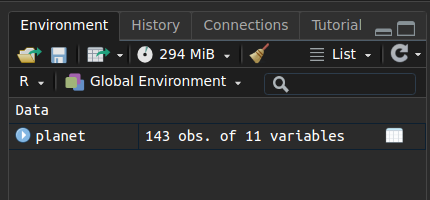
\includegraphics[keepaspectratio]{https://collinn.github.io/pics/planet_1.png}}

If we click on the blue arrow to the left, we will get a drop down
showing us a more detailed description of the variables we do have. Note
also the additional information given about the vectors (num = numeric,
int = integer, chr = character).

\pandocbounded{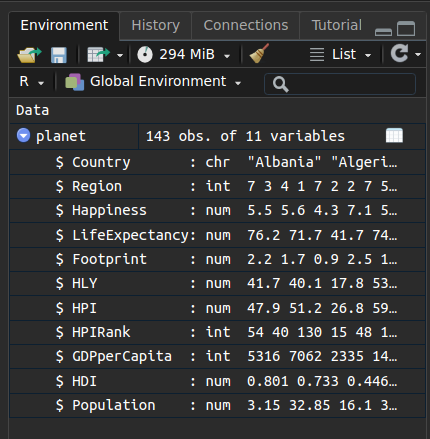
\includegraphics[keepaspectratio]{https://collinn.github.io/pics/planet_2.png}}

This information can also be produced by using the function str (for
structure).

\begin{Shaded}
\begin{Highlighting}[]
\FunctionTok{str}\NormalTok{(planet)}
\end{Highlighting}
\end{Shaded}

\begin{verbatim}
## 'data.frame':    143 obs. of  11 variables:
##  $ Country       : chr  "Albania" "Algeria" "Angola" "Argentina" ...
##  $ Region        : int  7 3 4 1 7 2 2 7 5 7 ...
##  $ Happiness     : num  5.5 5.6 4.3 7.1 5 7.9 7.8 5.3 5.3 5.8 ...
##  $ LifeExpectancy: num  76.2 71.7 41.7 74.8 71.7 80.9 79.4 67.1 63.1 68.7 ...
##  $ Footprint     : num  2.2 1.7 0.9 2.5 1.4 7.8 5 2.2 0.6 3.9 ...
##  $ HLY           : num  41.7 40.1 17.8 53.4 36.1 63.7 61.9 35.4 33.1 40.1 ...
##  $ HPI           : num  47.9 51.2 26.8 59 48.3 ...
##  $ HPIRank       : int  54 40 130 15 48 102 57 85 31 104 ...
##  $ GDPperCapita  : int  5316 7062 2335 14280 4945 31794 33700 5016 2053 7918 ...
##  $ HDI           : num  0.801 0.733 0.446 0.869 0.775 0.962 0.948 0.746 0.547 0.804 ...
##  $ Population    : num  3.15 32.85 16.1 38.75 3.02 ...
\end{verbatim}

\begin{Shaded}
\begin{Highlighting}[]
\CommentTok{\#an alternative is the head() fucntion which produces the first six rows of the data frame but won\textquotesingle{}t return the classes of the variables}

\FunctionTok{head}\NormalTok{(planet) }
\end{Highlighting}
\end{Shaded}

\begin{verbatim}
##     Country Region Happiness LifeExpectancy Footprint  HLY   HPI HPIRank
## 1   Albania      7       5.5           76.2       2.2 41.7 47.91      54
## 2   Algeria      3       5.6           71.7       1.7 40.1 51.23      40
## 3    Angola      4       4.3           41.7       0.9 17.8 26.78     130
## 4 Argentina      1       7.1           74.8       2.5 53.4 58.95      15
## 5   Armenia      7       5.0           71.7       1.4 36.1 48.28      48
## 6 Australia      2       7.9           80.9       7.8 63.7 36.64     102
##   GDPperCapita   HDI Population
## 1         5316 0.801       3.15
## 2         7062 0.733      32.85
## 3         2335 0.446      16.10
## 4        14280 0.869      38.75
## 5         4945 0.775       3.02
## 6        31794 0.962      20.40
\end{verbatim}

\begin{Shaded}
\begin{Highlighting}[]
\CommentTok{\#this is one of my most used functions}
\end{Highlighting}
\end{Shaded}

Clicking on the white box pane to the right of \texttt{planet} brings us
to the tabular view in R, giving us the opportunity to navigate and
explore the data more directly

\pandocbounded{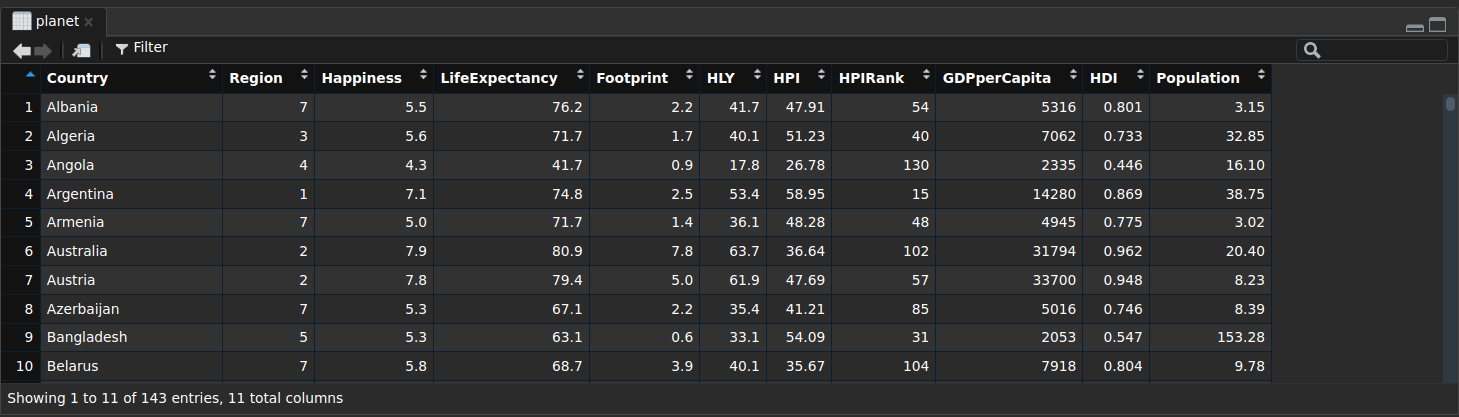
\includegraphics[keepaspectratio]{https://collinn.github.io/pics/planet_3.png}}

\textbf{Question 3:}

For this question, we will be using the \texttt{HappyPlanet} data that
we have just looked at:

\begin{itemize}
\item
  \textbf{Part A} Copy the code above to read the Happy Planet data into
  your own R Markdown file, saving the dataset to a variable called
  \texttt{planet}
\item
  \textbf{Part B} Looking at the Happy Planet data, explain in one or
  two sentences what constitutes an observation in this dataset (what is
  the data being recorded from)
\item
  \textbf{Part C} Using \texttt{\$} to extract columns from the dataset,
  find the mean life expectancy of all countries in the dataset? (Hint:
  what functions have we seen already in this lab?)
\item
  \textbf{Part D} Using {[},{]} to extract columns, what is the median
  GDP per Capita?
\item
  \textbf{Part E} Are there any variables in this dataset that are
  stored as a numeric that would be better suited as a categorical
  variable? Explain your answer
\end{itemize}

\begin{center}\rule{0.5\linewidth}{0.5pt}\end{center}

\begin{center}\rule{0.5\linewidth}{0.5pt}\end{center}

\subsection{Wrapping Up}\label{wrapping-up}

This concludes our first introduction to R. Once you have finished with
your lab, make sure that you are able to successfully Knit to PDF. Once
that is finished, we are ready to submit to canvas

\end{document}
